% Chapter 4: Operator Approximation Theory and Universality
% Part I of the book.

\chapter{Operator Approximation Theory and Universality}
\label{ch:part1-operator-approximation-theory-and-universa}
\label{sec:universality}
% -----------------------------------------------------------------------------

\chapref{ch:part1-partial-differential-equations-as-solution} closed with a catalogue of objects that no classical discretization delivers cheaply: the Darcy permeability-to-solution map, the Burgers and Navier--Stokes time-evolution maps. Each is a bounded, and in several cases smoothing, operator $\mathcal{G}:\mathcal{A}\to\mathcal{U}$ between infinite-dimensional function spaces.\index{solution operator} The rest of this part constructs candidate surrogates for such maps, and the question that ought to precede all of that engineering is whether a surrogate can exist at all: can a map specified by finitely many real parameters reach a continuous operator between function spaces to any prescribed accuracy? Universality theory answers in the affirmative; this chapter establishes the answer.

The problem is markedly harder than its finite-dimensional counterpart. A parameterized network carries $q$ degrees of freedom, where $\theta\in\mathbb{R}^{q}$; its target carries infinitely many, and requiring uniform accuracy over a whole class of input functions compounds the mismatch. \chapref{ch:part1-function-spaces-duality-and-sobolev-regula} and \chapref{ch:part1-partial-differential-equations-as-solution} have already isolated the escape route. Bounded sets in infinite dimensions fail to be precompact, so no finite-parameter family can approximate on a set as large as a ball of $L^{2}(\Omega)$; yet PDE solution operators do not act on such balls. They act on sets made compact by Sobolev regularity --- the Rellich--Kondrachov injection, the Darcy energy estimate, viscous smoothing in Burgers flow, the finite-dimensional global attractor of two-dimensional Navier--Stokes.\index{Burgers equation!viscous smoothing}\index{Navier--Stokes equations!smoothing and attractors} Compactness is therefore not a stylistic convenience of the theorems below but the physical content of the hypotheses made about solution operators.\index{compact set!approximation on}

Three results organize the chapter, in historical and in logical order. Chen and Chen's theorem of 1995 settles approximability for operators defined on compact subsets of a Banach space of continuous functions, and exposes a two-stage structure --- finitely many readings of the input, then a finite expansion in output functions --- which \textbf{DeepONet} (Deep Operator Network) converts into a trainable architecture.\index{Chen and Chen theorem}\index{universal approximation!for operators} The error analysis of Lanthaler, Mishra, and Karniadakis then prices those stages separately and isolates the residual left to the network. Finally, the generic neural operator of Kovachki et al.\ discards fixed sensor readings altogether and parameterizes a nonlocal integral kernel, with a universality theorem of its own.\index{neural operator!generic framework} The route taken here presupposes comfort with Sobolev spaces $H^{s}$, compact embeddings, the duality pairing $\langle\cdot,\cdot\rangle_{X^{*},X}$, and the notion of a continuous operator between Banach spaces, all supplied in \chapref{ch:part1-function-spaces-duality-and-sobolev-regula}; nothing beyond those tools is used. A closing section takes inventory of what none of the three theorems asserts --- the cost of evaluating the approximating operator, the absence of a rate linking $\varepsilon$ to the parameter budget, and the silence about training --- because that inventory drives everything that follows in Part I.

% -----------------------------------------------------------------------------
\section{The Classical Chen \& Chen Theorem (1995)}
% -----------------------------------------------------------------------------

Universal approximation theorems in the lineage of Cybenko, Hornik, and Pinkus~\cite{cybenko1989approximations} assert that a feedforward network with one hidden layer and a fixed non-polynomial activation can approximate any continuous \emph{function} of a finite-dimensional vector, uniformly on compact subsets of its input space. Chen and Chen lifted the statement from functions to \emph{operators} in 1995~\cite{chen1995universal}, keeping the three ingredients --- point evaluations, one nonlinear layer, one output expansion --- but relocating them between function spaces.

\begin{theorem}[Universal Approximation of Nonlinear Operators \cite{chen1995universal}]
\label{thm:chen_chen}
Let $K_{\mathrm{in}} \subset \mathbb{R}^{d_{\mathrm{in}}}$ and $K_{\mathrm{out}} \subset \mathbb{R}^{d_{\mathrm{out}}}$ be compact sets, and let $K_1$ be a compact subset of $C(K_{\mathrm{in}})$: the input and output domains are independent compacta, which is what makes the theorem usable for maps between functions on different sets. Let $\mathcal{G} : K_1 \to C(K_{\mathrm{out}})$ be a continuous nonlinear operator. Let $\sigma : \mathbb{R} \to \mathbb{R}$ be a continuous, non-polynomial activation function.

Then, for any $\varepsilon > 0$, there exist positive integers $m, n, p \in \mathbb{N}$, sensor locations $\{x_j\}_{j=1}^m \subset K_{\mathrm{in}}$, coefficients $c_k^i, \xi_{j}^i, \theta_i \in \mathbb{R}$, and continuous functions $\{g_k\}_{k=1}^p$ on $K_{\mathrm{out}}$ such that:
\begin{equation}
  \label{eq:chen_chen_form}
  \left| \mathcal{G}(u)(y) - \sum_{k=1}^p \sum_{i=1}^n c_k^i \, \sigma\left( \sum_{j=1}^m \xi_j^i \, u(x_j) + \theta_i \right) g_k(y) \right| < \varepsilon
\end{equation}
holds uniformly for all $u \in K_1$ and all $y \in K_{\mathrm{out}}$.
\end{theorem}

The shape of \eqref{eq:chen_chen_form} repays close reading, because every term in it reappears in the architectures that follow. Fix a hidden unit $i$ --- the index $i$ runs over the $n$ hidden units, a count distinct from the sensor number $m$ and the basis size $p$ --- and look first at $\sum_{j}\xi_{j}^{i}u(x_{j})+\theta_{i}$. The input function $u$ reaches the approximation \emph{only} through the $m$ scalar readings $u(x_{1}),\dots,u(x_{m})$; the weights $\xi_{j}^{i}$ collapse those readings to a single number, and $\sigma$ turns the number into one nonlinear feature. The coefficients $c_{k}^{i}$ then map the $n$ features into $p$ input-dependent amplitudes, and the family $\{g_{k}\}_{k=1}^{p}$ of continuous functions of the output coordinate $y$ performs the decoding. Written as $\sum_{k}b_{k}(u)g_{k}(y)$ with $b_{k}(u)=\sum_{i}c_{k}^{i}\sigma(\sum_{j}\xi_{j}^{i}u(x_{j})+\theta_{i})$, the right-hand side of \eqref{eq:chen_chen_form} is a rank-$p$ sum of separable terms, each the product of a functional of the input and a function of the output coordinate. That factorization, not the network wrapped around it, is the mathematical content of the theorem, and it is the structure DeepONet exploits in the next section.

Two hypotheses deserve comment.\index{activation function!non-polynomial} The activation is required only to be continuous and non-polynomial: no sigmoid, no smoothness, no monotonicity, and no boundedness is imposed, which sets the 1995 statement apart from the earliest finite-dimensional results, where the activation was fixed to be sigmoidal. The published form of the theorem writes the outer structure as a single sum $\sum_{k} c_k \sigma(\sum_j \xi_j^k u(x_j) + \theta_k) g_k(y)$; the double sum of \eqref{eq:chen_chen_form}, in which $n$ features are shared across $p$ basis functions, follows from it by re-indexing the pairs $(k,i)$ and allowing the basis to repeat, and it is stated this way because the shared-feature layout is the one DeepONet keeps. The set $K_{1}$ must be compact in $C(K_{\mathrm{in}})$, and the inequality is uniform over $K_{1}\times K_{\mathrm{out}}$, so one choice of $m$, $p$, and weights serves every input in $K_{1}$ at every output coordinate. Neither requirement is decorative. A family with finitely many parameters can $\varepsilon$-approximate only sets of finite metric entropy, and a closed bounded set in an infinite-dimensional space has infinite entropy --- the obstruction \chapref{ch:part1-function-spaces-duality-and-sobolev-regula} records through the Kolmogorov--Riesz and Arzel\`{a}-Ascoli criteria. What makes the theorem usable for PDEs is that the data pipeline supplies compact sets at both ends. On the input side, what discharges $K_{1}$'s compactness is an ensemble confined to a sublevel set of a stronger norm: the margin must clear the $s > d/2$ sensor threshold derived in \chapref{ch:part1-function-spaces-duality-and-sobolev-regula} through \eqref{eq:ch02-eval}, and then the Rellich--Kondrachov compactness recorded in \chapref{ch:part1-function-spaces-duality-and-sobolev-regula} turns the sublevel set into a compact set in the space the sensors see; ensembles whose only sublevel sets fall below that threshold --- the log-normal coefficient fields of Part~II, whose point values therefore fail to exist --- are reached by the measure-based reformulation of \cite{lanthaler2022error} rather than by this form of the theorem. On the output side the Darcy estimate bounds the image in $H^{1}_{0}(\Omega)$, and the same embedding renders it precompact in $L^{2}(\Omega)$, and in $C(\overline{\Omega})$ once the available Sobolev order exceeds $d/2$; viscous smoothing and the Navier--Stokes attractor yield compactness by different mechanisms. The compactness hypothesis is a statement about the PDE and its data, not about the network.\index{metric entropy}

The limits of \eqref{eq:chen_chen_form} as a working guide are equally worth stating. The result is existential. It produces no bound on $m$, $p$, or $n$ as a function of $\varepsilon$, so it cannot tell the practitioner how many sensors a Darcy problem needs for one percent error; it supplies no procedure for choosing the locations $\{x_{j}\}$; it offers no guarantee that the coefficients can be recovered from data by any optimization method; and it says nothing about inputs outside $K_{1}$. The first two gaps are confronted below: the error decomposition of the next section prices the sensor budget explicitly, and the same analysis accommodates randomly placed sensors, which is as much guidance as theory currently offers on the choice of $\{x_{j}\}$. The third gap is empirical and returns in Part II. The fourth is handled for DeepONets by the measure-based reformulation of~\cite{lanthaler2022error}, which extends the approximation property to measurable mappings on non-compact sets at the price of replacing the uniform norm with an $L^{2}$ norm in the input measure.

% -----------------------------------------------------------------------------
\section{The DeepONet Architecture}
% -----------------------------------------------------------------------------

Lu et al.~\cite{lu2021learning} turned the representation in \eqref{eq:chen_chen_form} into a deep architecture by keeping its separable skeleton and learning both halves.\index{DeepONet} \textbf{DeepONet} consists of two parallel subnetworks whose outputs are combined by an inner product. The \emph{branch network} ingests the vector of sensor evaluations $[u(x_1),u(x_2),\dots,u(x_m)]^{T}\in\mathbb{R}^{m}$ and returns a latent feature vector $\mathbf{b}(u)=[b_1(u),\dots,b_p(u)]^{T}\in\mathbb{R}^{p}$; it stands in for the double sum over hidden units and coefficients, and is free to be far deeper than one layer. The \emph{trunk network} ingests an arbitrary query coordinate $y\in\Omega$ and returns $\mathbf{t}(y)=[t_1(y),\dots,t_p(y)]^{T}\in\mathbb{R}^{p}$, learning the role that the fixed functions $\{g_{k}\}_{k=1}^{p}$ play in the Chen--Chen construction.\index{DeepONet!branch network}\index{DeepONet!trunk network} Read side by side, \eqref{eq:chen_chen_form} and \eqref{eq:ch04-deeponet} agree exactly at the level of the amplitudes: the branch output $b_{k}(u)$ replaces $\sum_{i}c_{k}^{i}\sigma(\sum_{j}\xi_{j}^{i}u(x_{j})+\theta_{i})$, and the trunk output $t_{k}(y)$ replaces $g_{k}(y)$. The network gains flexibility in both factors and inherits from the theorem the requirement that the two be summed in lockstep over the same index $k$, so branch width and trunk width are the same integer $p$. The approximation itself is the resulting inner product, augmented by an optional scalar bias $b_{0}\in\mathbb{R}$:
\begin{equation}
  \label{eq:ch04-deeponet}
  \mathcal{G}_\theta(u)(y) = \sum_{k=1}^p b_k\big( u(x_1), \dots, u(x_m) \big) \, t_k(y) + b_0 = \langle \mathbf{b}(u), \mathbf{t}(y) \rangle_{\mathbb{R}^p} + b_0.
\end{equation}
Because the two halves are decoupled, one pass through the branch serves every query point: a model evaluated at $N_{\mathrm{q}}$ query coordinates costs one branch pass, $N_{\mathrm{q}}$ inexpensive trunk passes, and a rank-$p$ contraction, so the work per query grows linearly in the sensor count $m$ and the basis size $p$ rather than quadratically in a grid of $N$ nodes (compare the complexity row of \chapref{ch:part1-comparative-theoretical-taxonomy-of-archit}).

The asymmetry inside \eqref{eq:ch04-deeponet} is the architecture's defining feature and its main practical restriction. The output side is coordinate-free: $y$ is an argument of the trunk network, so a trained model can be queried at points never seen during training. The input side is not: $u$ enters through $m$ slots at prescribed locations $\{x_{j}\}_{j=1}^{m}$, so every new input function must be sampled at those same sensors for the branch output to remain meaningful. DeepONet is thus invariant under changes of the \emph{output} discretization while remaining tied to a fixed \emph{input} measurement set --- the distinction \chapref{ch:part1-comparative-theoretical-taxonomy-of-archit} records in its discretization-invariance row, and panel (b) of Figure~\ref{fig:architectures} makes visible.

\begin{remark}[DeepONet error decomposition, after \cite{lanthaler2022error}]
\label{thm:deeponet_error}
Let $\mathcal{G}: \mathcal{A} \to \mathcal{U}$ be a Hölder-continuous operator between Sobolev spaces with essentially relatively compact range, let the inputs be drawn from a probability measure $\mu$ on $\mathcal{A}$, and let $\mathcal{G}_\theta$ be a DeepONet with $m$ sensors, trunk rank $p$, and branch and trunk networks of depth $L$ and widths $d_b$, $d_t$. The error analyzed in \cite{lanthaler2022error} is measured in $L^{2}(\mu)$, and its bound separates into three contributions of different character:
\begin{equation}
  \label{eq:ch04-error-split}
  \Big( \mathbb{E}_{u \sim \mu} \big\| \mathcal{G}(u) - \mathcal{G}_\theta(u) \big\|_{\mathcal{U}}^{2} \Big)^{1/2}
  \;\lesssim\;
  \mathcal{E}_{\text{sensor}}(m) + \mathcal{E}_{\text{basis}}(p) + \mathcal{E}_{\text{DNN}}(L, d_b, d_t),
\end{equation}
where $\mathcal{E}_{\text{sensor}}(m)$ is the encoding error incurred by reading $u$ through $m$ discrete sensors, $\mathcal{E}_{\text{basis}}(p)$ is the approximation error of the rank-$p$ trunk expansion, and $\mathcal{E}_{\text{DNN}}(L, d_b, d_t)$ is the reconstruction error of implementing branch and trunk by networks of depth $L$ and widths $d_b$, $d_t$. The symbol $\lesssim$ hides the continuity constants of $\mathcal{G}$; in the original statement the encoding term enters to the Hölder power rather than additively, and the display is the taxonomy the source's bounds support, not a theorem proved in this book. Note that $\theta$ enters only through the architecture sizes it indexes: the split prices the class, not any particular training outcome.
\end{remark}

The three terms of \eqref{eq:ch04-error-split} are additive, and each answers a question about a different design choice.\index{DeepONet!error decomposition}\index{sensor placement} The sensor term is charged before any learning begins: it is the price of compressing $u$ to $m$ numbers, and it falls only when the input ensemble is efficiently encodable, which is again a regularity property of the measure carried by $\mathcal{A}$. The basis term is a width question about the output set --- how well $p$ functions from the trunk can span the range of $\mathcal{G}$ --- and it shrinks quickly for smooth outputs, whose energy concentrates in few modes. The last term is a budget question about the two networks --- how well branch and trunk of a given depth and width can realize the maps the first two terms ask of them --- and it shrinks as $L$, $d_b$ or $d_t$ grow; nothing in it refers to any particular training run. What training does add, and what no term of \eqref{eq:ch04-error-split} prices, is the gap between the best parameters of the class and the parameters an optimizer returns; that gap lives outside the display and is confronted empirically in Part~II.

In the analysis of~\cite{lanthaler2022error} these contributions appear under the names encoding, approximation, and reconstruction errors; upper and lower bounds on the total are expressed through the spectral decay of the covariance operators associated with the underlying measures, very general affine reconstructions are admitted on the output side, sensors may be placed at random rather than tuned by hand, and generalization is controlled through covering-number arguments.\index{covering number} The value of \eqref{eq:ch04-error-split} in practice is therefore diagnostic rather than prescriptive: an error floor that refuses to move while the training loss still falls indicates a dominant $\mathcal{E}_{\text{sensor}}(m)$ or $\mathcal{E}_{\text{basis}}(p)$, that is, a budget problem in the sensors or the trunk width rather than an under-trained network.

% -----------------------------------------------------------------------------
\section{The Generic Neural Operator Framework}
% -----------------------------------------------------------------------------

DeepONet asks what a function \emph{is} at $m$ points. The framework of Kovachki et al.~\cite{kovachki2023neural} asks instead what the \emph{map} is, and answers by parameterizing an integral operator, so that the architecture acts on continuum functions and commits to no fixed measurement set. Its motivation is structural as much as computational: \chapref{ch:part1-partial-differential-equations-as-solution} showed that the inverse of a linear elliptic operator is an integral operator with Green's kernel $G_{a}(x,y)$, which suggests that a trainable kernel is the natural surrogate for a solution operator.\index{Green's function}

\begin{definition}[Generic Neural Operator Architecture \cite{kovachki2023neural}]
\label{def:generic_no}
Let $\mathcal{A} = \mathcal{A}(\Omega; \mathbb{R}^{d_a})$ and $\mathcal{U} = \mathcal{U}(\Omega; \mathbb{R}^{d_u})$ be function spaces over $\Omega \subset \mathbb{R}^d$. A Neural Operator $\mathcal{G}_\theta : \mathcal{A} \to \mathcal{U}$ is parameterized as:
\begin{equation}
  \label{eq:no_composition}
  \mathcal{G}_\theta = \mathcal{Q} \circ \mathcal{V}_L \circ \mathcal{V}_{L-1} \circ \dots \circ \mathcal{V}_1 \circ \mathcal{P},
\end{equation}
where $\mathcal{P} : \mathbb{R}^{d_a} \to \mathbb{R}^{d_v}$ is a local, pointwise lifting operator, typically parameterized by a shallow multilayer perceptron (MLP) acting on channel dimensions, so that $v_0(x) = \mathcal{P}(a(x))$. The hidden layers $\mathcal{V}_\ell : v_\ell \mapsto v_{\ell+1}$ are non-local and defined by
\begin{equation}
  \label{eq:no_layer}
  v_{\ell+1}(x) = \sigma\left( W_\ell v_\ell(x) + \big(\mathcal{K}_\ell(a; \phi_\ell) v_\ell\big)(x) + b_\ell(x) \right), \quad \ell = 0, \dots, L-1,
\end{equation}
in which $W_\ell \in \mathbb{R}^{d_v \times d_v}$ is a local linear transformation, $b_\ell \in C(\Omega; \mathbb{R}^{d_v})$ is a bias function, $\sigma : \mathbb{R} \to \mathbb{R}$ is an element-wise activation function, and $\mathcal{K}_\ell$ is a Fredholm integral kernel operator, built from a kernel whose trainable parameters are collected in $\phi_\ell$:
\begin{equation}
  \label{eq:fredholm_kernel}
  \big(\mathcal{K}_\ell(a; \phi_\ell) v_\ell\big)(x) = \int_\Omega \kappa_\ell(x, y, a(x), a(y); \phi_\ell) \, v_\ell(y) \, dy.
\end{equation}
The final ingredient $\mathcal{Q} : \mathbb{R}^{d_v} \to \mathbb{R}^{d_u}$ is a local, pointwise projection operator mapping hidden representations back to physical solution channels, $u(x) = \mathcal{Q}(v_L(x))$.
\end{definition}

Every object in Definition~\ref{def:generic_no} is a function of continuum variables, and that is the point of the construction.\index{lifting operator}\index{projection operator}\index{$d_v$, hidden channel width} The lifting stage $\mathcal{P}$ in \eqref{eq:no_composition} applies one shallow MLP to the $d_{a}$ physical channels of $a$ at each point and returns $d_{v}$ hidden channels: a scalar permeability field becomes a $d_{v}$-component latent field with no mixing of neighbors. Mixing is deferred to the single nonlocal ingredient of \eqref{eq:no_layer}, the operator $\mathcal{K}_{\ell}$ defined by \eqref{eq:fredholm_kernel}, which couples every pair of points in $\Omega$. The division of labor is not cosmetic. A pointwise map --- $\mathcal{P}$, $\mathcal{Q}$, $W_{\ell}$, $b_{\ell}$ --- can rescale and rotate channels but cannot carry information from $y$ to $x$, so a stack of such layers applied to a coefficient field could never reproduce the global redistribution of mass, momentum, or flux that \chapref{ch:part1-partial-differential-equations-as-solution} attributes to a Green's kernel. A purely linear integral operator, on the other hand, cannot generate the shock steepening of Burgers flow. Alternating the two $L$ times, as \eqref{eq:no_layer} prescribes, yields a class large enough for the universality statement below while leaving each layer interpretable: the local part carries pointwise constitutive behavior, the nonlocal part carries long-range coupling. Note finally the argument list of the kernel $\kappa_{\ell}$ in \eqref{eq:fredholm_kernel}, a function of $(x,y,a(x),a(y))$; dependence on the input values at both endpoints is what lets the layer condition its own long-range interactions on the coefficient field, and it is exactly what a convolution, whose kernel sees only $x-y$, cannot do.\index{Fredholm integral operator}\index{integral kernel!parameterized}

\begin{theorem}[Universal Approximation of Neural Operators \cite{kovachki2023neural}]
\label{thm:no_universality}
Let $\Omega \subset \mathbb{R}^d$ be compact, let $r > d/2$, and let $\mathcal{A} = H^r(\Omega; \mathbb{R}^{d_a})$ and $\mathcal{U} = L^2(\Omega; \mathbb{R}^{d_u})$. Let $K \subset \mathcal{A}$ be a compact subset, and let $\mathcal{G} : K \to \mathcal{U}$ be a continuous (possibly nonlinear) operator. The regularity margin is not decorative: $r > d/2$ embeds the inputs in $C(\overline{\Omega})$, which is what makes the kernel's endpoint evaluations $a(x), a(y)$ in \eqref{eq:fredholm_kernel} meaningful; for $K \subset L^2$ the statement below holds only for the subclass of kernels of $(x,y)$ alone.

Assume the activation function $\sigma$ is non-polynomial and Lipschitz continuous. Then, for any $\varepsilon > 0$, there exist an integer $L \ge 1$, a channel dimension $d_v$, a lifting map $\mathcal{P}$ and projection map $\mathcal{Q}$ of \eqref{eq:no_composition}, parameters $\{W_\ell, b_\ell\}$, and continuous kernel functions $\kappa_\ell \in C(\Omega \times \Omega \times \mathbb{R}^{d_a} \times \mathbb{R}^{d_a}; \mathbb{R}^{d_v \times d_v})$, matched to the input-conditioned class of \eqref{eq:fredholm_kernel}, such that the neural operator $\mathcal{G}_\theta$ defined in \eqref{eq:no_composition}--\eqref{eq:fredholm_kernel} satisfies:
\begin{equation}
  \label{eq:ch04-unif-bound}
  \sup_{a \in K} \|\mathcal{G}(a) - \mathcal{G}_\theta(a)\|_{L^2(\Omega; \mathbb{R}^{d_u})} < \varepsilon.
\end{equation}
\end{theorem}

Theorem~\ref{thm:no_universality} shares the anatomy of Theorem~\ref{thm:chen_chen} --- compact domain, continuous target, non-polynomial activation --- but the bound \eqref{eq:ch04-unif-bound} is stated in the $L^{2}$ norm rather than the uniform norm, which suits measurable targets and the Sobolev hierarchies used later in Part I, and it leaves both the depth $L$ and the width $d_{v}$ to the existence argument instead of fixing a one-hidden-layer form. The theorem's kernel class is the input-conditioned one of \eqref{eq:fredholm_kernel}, and the margin $r > d/2$ is what licenses it: with pointwise-defined inputs there is no gap left between the class the bound quantifies over and the layers that are actually implemented. The proof strategy is worth tracing, because it says what integral parameterization is for. First, compactness makes the image of $K$ coverable by finitely many balls of radius $\varepsilon$, so $\mathcal{G}$ is uniformly approximable on $K$ by a finite-rank map whose coefficients are continuous functionals of the whole input field. Second, those functionals are of a kind the kernel layer can realize --- integral expressions $\int_\Omega \kappa(x, y)\, a(y) \, dy$ against fixed representers --- and it is the $(x,y)$-dependence of the kernel, not the input conditioning, that the separable-sum density supplied by the Stone--Weierstrass theorem addresses. Third, the composed pointwise operations on the finitely many resulting channel values fall to the classical Cybenko construction.\index{Stone--Weierstrass theorem}\index{Cybenko theorem}\index{universal approximation!neural operator} Applying \eqref{eq:no_composition} to fields rather than to vectors is what separates this argument from its finite-dimensional ancestor: every ingredient operates on functions, so the approximating object is itself an operator and not a map handed a discretization.

Figure~\ref{fig:architectures} collects the feedforward family, the branch--trunk design of \eqref{eq:ch04-deeponet}, and the spectral variant that opens \chapref{ch:part1-the-fourier-neural-operator-spectral-theor}, and the comparison it invites is sharper than a gallery of boxes. In panel (a), the multilayer perceptron and the convolutional network consume a vector of samples on a fixed mesh $\mathcal{M}_{N}$ of $N$ grid points, so the parameter count is tied to $N$ and the trained weights lose their meaning when the grid changes; neither resolution transfer nor querying at new coordinates is available without interpolation. In panel (b), DeepONet separates the two roles that \eqref{eq:chen_chen_form} couples: the branch network is bound to $m$ input sensors, while the trunk accepts any continuous $y\in\Omega$, and the inner product of \eqref{eq:ch04-deeponet} fuses them, which buys a resolution-free output at the cost of a fixed input measurement set. In panel (c), the Fourier neural operator (FNO) of \cite{li2021fourier} keeps the lift-and-project sandwich of \eqref{eq:no_composition} but replaces the dense kernel of \eqref{eq:fredholm_kernel} with a spectral convolution, so its parameters attach to frequency modes rather than to grid indices and one trained map applies to every discretization of the periodic domain. Read in that order, the panels isolate a single axis of difference: \emph{what the parameters are functions of} --- grid indices, sensor slots, or wavenumbers.

\begin{figure}[t]
\centering
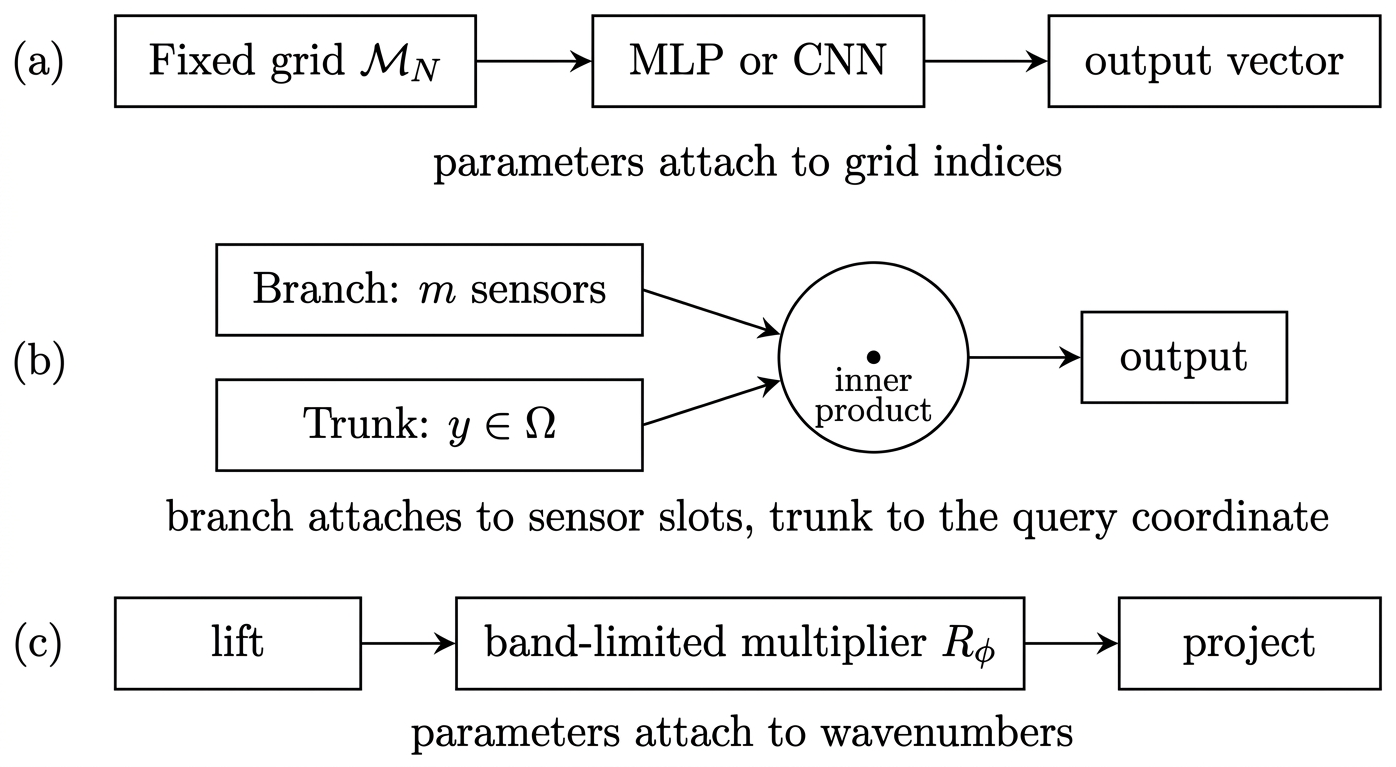
\includegraphics[width=0.82\textwidth]{fig_architectures.png}
\caption{\textbf{Three architectural families, as block diagrams.} (a) A multilayer perceptron or convolutional network consumes a vector of samples on a fixed mesh $\mathcal{M}_{N}$, so its parameters attach to grid indices. (b) DeepONet separates the two roles that \eqref{eq:chen_chen_form} couples: a branch bound to $m$ input sensors, a trunk accepting any continuous $y\in\Omega$, fused by the inner product of \eqref{eq:ch04-deeponet}. (c) The Fourier neural operator \cite{li2021fourier} keeps the lift-and-project sandwich of \eqref{eq:no_composition} but replaces the dense kernel of \eqref{eq:fredholm_kernel} with a spectral convolution, so its parameters attach to wavenumbers. Read in that order the panels isolate one axis of difference: what the parameters are functions of. The plate is a schematic rendering of the constructions defined in this chapter and carries no measured value.}
\label{fig:architectures}
\end{figure}

% -----------------------------------------------------------------------------
\section{What the Universality Theorems Do Not Say}
% -----------------------------------------------------------------------------

Put in sequence, Theorems~\ref{thm:chen_chen} and~\ref{thm:no_universality}, together with the error taxonomy of Remark~\ref{thm:deeponet_error}, deliver a reassuring conclusion: no architecture family considered here is fundamentally unable to represent a PDE solution operator. Three questions remain open, and each reappears later in the book.

The first is cost. Discretizing \eqref{eq:fredholm_kernel} on $N$ nodes forms an $N\times N$ kernel matrix, so a densely parameterized layer is $\mathcal{O}(N^{2})$ in time and memory, which is prohibitive in two and three dimensions. The contraction \eqref{eq:ch04-deeponet} carries no such bottleneck, because a rank-$p$ sum is cheap, but its expressivity is capped by the same $p$ that governs $\mathcal{E}_{\text{basis}}(p)$ in \eqref{eq:ch04-error-split}. The generic framework of~\cite{kovachki2023neural} admits several tractable kernel parameterizations in response --- graph-based, low-rank, multipole, and Fourier~\cite{li2021fourier} --- each buying efficiency by restricting the kernel's dependence on $(x,y)$, and each restriction must then earn back the accuracy it forfeits. Theorem~\ref{thm:no_universality} cannot say which restriction is worthwhile; that is an architectural question, and Part I answers it for the Fourier case.

The second is rate. An existential theorem supplies a family of approximators but no map from $\varepsilon$ to $(L,d_{v},p,m)$, so it cannot distinguish an architecture needing parameters polynomial in $1/\varepsilon$ from one needing them exponentially large --- and a surrogate whose size explodes with accuracy is useless in practice. Bounds of this kind do exist for the two architectures that dominate the rest of the book. For DeepONets, \cite{lanthaler2022error} control the three contributions in \eqref{eq:ch04-error-split} through the spectral decay of the covariance operators of the input and output measures, converting the bare requirement ``$K$ is compact'' into a computable statement about how fast the leading coefficients of the data ensemble decay. For Fourier neural operators, \cite{kovachki2021universal} prove universality together with explicit error bounds, and show that for the solution operators of Darcy flow and of the incompressible Navier--Stokes equations the network size required to reach error $\varepsilon$ grows only sub-log-linearly in $1/\varepsilon$ --- efficiency in precisely the sense the existential results above decline to provide.\index{Darcy flow!approximation}\index{Navier--Stokes equations!approximation}\index{universality!versus efficiency}\index{Fourier neural operator!error bounds}

The third is training. Every result in this chapter is a statement about a hypothesis class. None asserts that stochastic gradient descent finds a member of it, that empirical risk on a finite training set controls the supremum in \eqref{eq:ch04-unif-bound} over $K$, or that the loss landscape is benign. All three terms of \eqref{eq:ch04-error-split} are class-level quantities --- sensors, basis, network size --- and none is a statement about optimization; the gap the split omits lives outside it. This chapter has kept them apart deliberately: generalization and stability are taken up in \chapref{ch:part1-open-theoretical-problems-and-mathematical}, their empirical counterpart in Part II. What universality does accomplish is narrower and sufficient to justify everything that follows. Where the hypotheses of the three theorems hold --- a target that is continuous on a compact input set --- a neural operator that fails on a PDE family fails in the budget, the parameterization, the data, or the optimizer, not in the representability of the target. Where those hypotheses fail, as they do for a transport map that propagates a discontinuity without smoothing it, the theorems make no promise at all, and \chapref{ch:part1-open-theoretical-problems-and-mathematical} records that as an open problem rather than a solved one.\index{universality!scope of the hypotheses}

% -----------------------------------------------------------------------------
% Bridge to Chapter 5
% -----------------------------------------------------------------------------

The unresolved item from the preceding section is the cost of the nonlocal term, and it is the reason \chapref{ch:part1-the-fourier-neural-operator-spectral-theor} exists. An $\mathcal{O}(N^{2})$ kernel integral is affordable only if the kernel's dependence on $(x,y)$ is restricted, so the question becomes what to give up. A translation-invariant kernel $\kappa(x-y)$ on a periodic domain surrenders the input conditioning visible in \eqref{eq:fredholm_kernel}, but it turns the integral of \eqref{eq:fredholm_kernel} into a convolution, and convolutions are diagonal in the Fourier basis. That single observation converts dense integration into per-mode multiplication by a learnable complex matrix, evaluated in $\mathcal{O}(N\log N)$ with a fast Fourier transform (FFT), and it relocates the parameters onto wavenumbers instead of grid indices --- the structural premise of the discretization-invariance analysis in \chapref{ch:part1-discretization-invariance-and-continuum-li}.\index{discretization invariance}\index{mesh independence|see{discretization invariance}} \chapref{ch:part1-the-fourier-neural-operator-spectral-theor} develops exactly that construction: Fourier multipliers and stationary kernels, mode truncation to a finite set $Z_{k_{\max}}$, the conjugate-symmetry constraint that keeps outputs real-valued, and the spectral layer \eqref{eq:fno_layer}, which replaces the integral in \eqref{eq:no_layer}. It then supplies the rate statement this chapter withheld, splitting the error into a spectral truncation part that decays algebraically in $k_{\max}$ and a neural parametric floor --- the analogue, in a frequency parameterization, of the basis term $\mathcal{E}_{\text{basis}}(p)$ in \eqref{eq:ch04-error-split}.
